\chapter{非合作博弈与拍卖机制相关理论基础}

\textbf{本章摘要:} 
本章分别介绍了与本文相关的非合作博弈的基本概念,包括动态博弈的分类、斯塔克伯格博弈模型;同时介绍了与本文相关的拍卖机制设计理论;最后介绍了行为经济学中展望理论框架下博弈中个体的非完全理性模型。


\textbf{关键词:}非合作博弈;拍卖机制设计;展望理论

%\section{引言}

\section{非合作博弈相关理论基础}\label{sec:game}
博弈论(Game Theory)是研究理性个体互动决策的理论,源于应用数学领域,后又在经济学、计算机科学、管理学等学科领域得到进一步理论发展与广泛应用。根据博弈参与者能否形成约束性协议,博弈可分为合作博弈和非合作博弈\cite{osborne,Fudenberg}。一般认为,当参与者根据自身利益,无法与其他参与者就行动选择达成约束性协议而独立作出决策时,该博弈模型属于非合作博弈\cite{osborne}。

\subsection{非合作博弈的表征}

非合作博弈的表征形式包含三类,即策略博弈(Strategic game)、延展博弈(Extensive game)和联合博弈(Coalitional game),在本文中我们的讨论主要是策略博弈\cite{osborne}。策略博弈是一种典型的静态博弈,其中所有的参与者同时进行行动,在数学上有如下的定义:
\begin{df}[策略博弈]
一个策略博弈可以由一个有序三元组定义:
\begin{equation}
\mathcal{G}=(\mathcal{V},\{\mathcal{S}_i\}_{i\in\mathcal{V}},\{u_i\}_{i\in\mathcal{V}})
\end{equation}
其中
\begin{enumerate}
\item $\mathcal{V}=\{1,\cdots,N\}$为一个有限的参与者集合。
\item $\mathcal{S}_i$为表示参与者$i$可行策略空间的一个非空策略集合。
\item $u_i: \mathcal{S}\rightarrow  \mathbb{R}$代表参与者$i$的收益,其中$\mathcal{S}\triangleq\prod_i\mathcal{S}_i$代表所有参与者的策略空间。
\end{enumerate}
\end{df}
根据上述定义,一个策略博弈模型可以由参与者集合、行为集合和参与者在不同行为交互情况下的收益集合三部分来表征。博弈的参与者其中当策略集合$\mathcal{S}_i$为由参与者$i$所有可选行动组成的集合$\mathcal{A}_i=(a_{i1},a_{i2},\cdots)$时,元素$s_i\in\mathcal{S}_i$也被称为纯策略(Pure-strategy)。对应地,当策略集合中的元素$s_i\in\mathcal{S}_i$对应于参与者$i$定义在可选行动集合$\mathcal{A}$上的一个策略分布$\pi_i$时,元素$s_i\in\mathcal{S}_i$则被称为一个混合策略(Mixed-strategy)。进一步,我们令向量$s_{-i}=[s_j]_{j\neq i}\in\mathcal{S}_{-i}$为除参与者$i$外其余参与者的策略向量,其中$\mathcal{S}_{-i}\triangleq\prod_{j\neq i}S_j$表示除参与者$i$外其余参与者的策略空间。


\subsection{博弈的均衡}\label{sec:neconcept}

最优响应是指博弈中参与者在其他参与者策略已知或可预测条件下,给自身带来最大化收益的策略\cite{osborne,Fudenberg},数学上定义如下:
\begin{df}[最优响应]
对于策略博弈$\mathcal{G}=(\mathcal{V},\{\mathcal{S}_i\}_{i\in\mathcal{V}},\{u_i\}_{i\in\mathcal{V}})$中的任意参与者$i\in\mathcal{V}$,及任意$s_{-i}\in\mathcal{S}_{-i}$,参与者$i$的最优响应为
\begin{equation}
B_i(s_{-i})=\arg\max_{s_i\in\mathcal{S}_i}u_i(s_i,s_{-i})
\end{equation}
\end{df}

当一个策略博弈中的每个参与者都将最优响应作为自己的行动时,该博弈即可达到均衡状态,对应的所有参与者的策略即为纳什均衡(Nash Equilibrium)\cite{Nash1951},其定义如下:
\begin{df}[纳什均衡]
假设对于策略博弈$\mathcal{G}=(\mathcal{V},\{\mathcal{S}_i\}_{i\in\mathcal{V}},\{u_i\}_{i\in\mathcal{V}})$中每个个体$i\in\mathcal{V}$,若满足
\begin{equation}\label{}
u_{i}(s_{i}^*,s_{-i}^*)\ge u_{i}(s_{i},s_{-i}^*),~\forall s_i\ne s_i^*.
\end{equation}
则纯策略$s^*=(s_{1}^*,\cdots,s_{N}^*)\in\mathcal{S}$是一个(纯策略)纳什均衡。
\end{df}
对于使用纳什均衡作为策略博弈的解,较为广泛的一种解释是因为纳什均衡对应于博弈的一个稳定状态,在这个状态上任何参与者都无法通过单方面改变其策略以获得更高的收益,因而没有偏离其当前均衡策略的动机。然而由于一个策略博弈并不能保证其纯策略纳什均衡的存在,因而出现了由纳什均衡衍生出的一些其他均衡概念,这些均衡解的出现方便了对于博弈模型均衡状态的分析。例如,当博弈中参与者所使用的策略$s_i$对应为一个混合策略$\pi_i\in\Delta\mathcal{A}$时,博弈相应的均衡即成为混合纳什均衡\cite{Fudenberg,Lasaulce2011}。
\begin{df}[混合纳什均衡]
假设对于策略博弈$\mathcal{G}=(\mathcal{V},\{\mathcal{S}_i\}_{i\in\mathcal{V}},\{u_i\}_{i\in\mathcal{V}})$中每个个体$i\in\mathcal{V}$,若满足
\begin{equation}\label{}
u_{i}(\pi_{i}^*,\pi_{-i}^*)\ge u_{i}(\pi_{i},\pi_{-i}^*) + \epsilon,~\forall \pi_i\ne\pi_i^*.
\end{equation}
则混合策略均衡$\pi^*=(\pi_{1}^*,\cdots,\pi_{N}^*)\in\Delta\mathcal{A}$是一个混合纳什均衡。
\end{df}

一个混合策略是对于参与者所有可能行为的随机化选择,因此不难理解纯策略纳什均衡是混合策略纳什均衡的一个特例。进一步我们还可以通过设定一个阈值$\epsilon$,更具一般性地得到对于混合策略纳什均衡的一个近似,即$\epsilon$-纳什均衡\cite{Fudenberg,Lasaulce2011}:
\begin{df}[$\epsilon$-纳什均衡]
假设对于策略博弈$\mathcal{G}=(\mathcal{V},\{\mathcal{S}_i\}_{i\in\mathcal{V}},\{u_i\}_{i\in\mathcal{V}})$中每个个体$i\in\mathcal{V}$,若满足
\begin{equation}\label{}
u_{i}(\pi_{i}^*,\pi_{-i}^*)\ge u_{i}(\pi_{i},\pi_{-i}^*) + \epsilon,~\forall \pi_i\ne\pi_i^*.
\end{equation}
则混合策略均衡$\pi^*=(\pi_{1}^*,\cdots,\pi_{N}^*)\in\Delta\mathcal{A}$是一个$\epsilon$纳什均衡。
\end{df}

当博弈处于$\epsilon$-纳什均衡状态时意味着任意参与者通过单方面偏离博弈均衡策略只能获得不超过$\epsilon$的收益增加。
%由于$\epsilon$-纳什均衡属于混合纳什均衡,因此一个有限博弈可以确保存在一个$\epsilon$-纳什均衡。
以上所介绍的纳什均衡相关概念中均默认要求参与者独立地完成策略(纯策略或混合策略)的选择。在一些情况下,博弈参与者的策略之间可能存在相关性。例如,当博弈开始前参与者之间存在一定的信息交互,或博弈存在一个“协调者”可以向每个参与者进行策略建议(参与者可以不接受)。在这种设定下,博弈的稳态可由相关均衡(Correlated Equilibrium)\cite{Aumann}来刻画:
\begin{df}[相关均衡]
我们称定义在$\Delta\mathcal{S}$上的联合概率分布$\pi^*$为一个非合作博弈$\mathcal{G}=(\mathcal{V},\{\mathcal{S}_i\}_{i\in\mathcal{V}},\{u_i\}_{i\in\mathcal{V}})$的一个相关均衡(CE),如果$\forall i\in\V$,$\forall t_{i},s_i\in\mathcal{S}_i$,$t_i\neq s_i$,个体收益$u_i$满足以下不等式,
%A probability distribution $\pi^*$ on $\Delta\mathcal{M}$ is a socially-aware correlated equilibrium (CE) of game $\Gamma$ if, $\forall n\in\V$, $\forall a_{n,i},a_{n,j}\in\mathcal{M}_n$, the expected group utility satisfies the following,
\begin{equation}
\sum_{s_{-i}\in\mathcal{S}_{-i}}\pi^*(s)\left[u_i(t_i,s_{-i})-u_i(s)\right]\leq0.
\end{equation}
\end{df}

在相关均衡状态上,任何参与者都无法通过单方面偏离“协调者”的建议而获得收益的提升。从以上定义可以看出,一个混合纳什均衡可以被看作为一个相关均衡的特例,因而相关均衡在实际中较混合纳什均衡更易出现。
%在一些不存在纯纳什均衡的有限博弈中,我们可以转而使用混合纳什均衡和相关均衡来研究分析博弈的均衡状态。
本文中第四章使用了相关均衡(CE)来刻画移动设备的频谱选择均衡策略,本文的第五章则分别使用了纳什均衡和$\epsilon$-纳什均衡的概念对于移动用户和服务提供商的均衡策略进行刻画。博弈论中还有其他的均衡概念,例如占优策略均衡(Dominant strategy Equilibrium)和子博弈精炼均衡(Subgame Perfect Equilibrium)和均衡等,由于他们在本文中没有涉及,这里我们不进行详细介绍。

博弈论中对于博弈均衡解的研究通常包括对于均衡解存在性、唯一性以及均衡解效率上的分析。从数学上讲,证明纳什均衡的存在等价于证明一个定点问题(Fixed-point problem)解的存在性。因此众多关于均衡存在证明的工作都基于对于定点定理的推导。本节仅介绍一个与本文相关的纳什均衡存在性的结论\cite{Nash48}。

%\begin{thm}(有限博弈中纯纳什均衡的存在性)
%在理想信息前提下,每一个有限博弈存在至少一个纯纳什均衡。
%\end{thm}

\begin{thm}[有限博弈中混合纳什均衡的存在性]
若策略博弈$\mathcal{G}=(\mathcal{V},\{\mathcal{S}_i\}_{i\in\mathcal{V}},\{u_i\}_{i\in\mathcal{V}})$满足参与者集合与对应的策略集合为有限集合,则称该博弈为有限博弈(Finite Game),且该博弈至少存在一个混合纳什均衡。
\end{thm}

博弈均衡解的唯一性与均衡解的质量相比存在性分析更为复杂,且通常需要在特定问题模型中针对具体问题进行具体分析,因此不在这里进行介绍。

%当一个动态博弈具有有限的状态空间与动作空间时,该动态博弈至少存在一个策略均衡。而通常一个存在均衡的动态博弈会同时拥有多个均衡状态。

\subsection{动态博弈}
非合作博弈模型可以被分为静态博弈与动态博弈两类\cite{osborne,Fudenberg,han2012game}。通常,我们认为静态博弈中参与者拥有对于博弈确定的认知,包括对于信息和行为的假设,且这些认知不随博弈进行而改变,参与者则仅需基于已有的关于其他参与者信息行为的假设进行一次性的行动。前几节中我们正是在静态博弈的范畴下对于策略博弈的表征形式与均衡概念进行了相关的讨论。相比于静态博弈,动态博弈中通常假设参与者可以从过往的行动和策略中提取有用信息,并用于当前与未来行动与策略的制定。动态博弈模型主要包括以下几类:

\begin{itemize}
\item {\heiti 重复博弈:}顾名思义,一个标准的重复博弈包含对于同一静态博弈有限或无限次的重复进行,其中参与者通过重复的策略交互以求最大化自身长期收益,会产生静态博弈中所不存在的合作与惩罚的现象。
\item {\heiti 随机博弈:}随机博弈则较重复博弈更具一般性。参与者的即时收益不单取决于当前参与者的行为,同时取决于环境当前的状态。随机博弈中又可细分为共同状态(Common states)随机博弈和个体状态(Individual states)随机博弈。共同状态随机博弈中博弈环境对于所有参与参与者相同,而在个体状态随机博弈中,每个参与者可以处于不同的博弈环境状态。
\item {\heiti 差分/差异博弈:}与重复博弈和随机博弈不同,差分/差异博弈则在时间上是连续的。通常,差分博弈中的状态进化规则(例如一个确定性的或者随机的差分方程)。差异博弈则是对于差分博弈的离散化,当处于极限情况下时即等价于差分博弈。差异博弈可被看作为介于差分博弈与随机博弈之间的一种动态博弈类型。
\item {\heiti 演化博弈:}演化博弈通常涉及到大规模的用户,侧重于研究用户间交互所导致的群体演化的研究。其应用起源于生物学与社会学中。
\end{itemize}

与静态博弈不同,动态博弈在建模中需考虑两个较为关键的问题:首先,如何对参与者所处的动态环境进行建模。一些差分方程用于从数学上刻画参与者所处环境的动态特性。其次,如何对参与者的目标进行建模。在大部分场景下,参与者的收益需要根据动态环境调整为长期的期望收益。本文的研究内容主要涉及到重复博弈与个体状态随机博弈。

\subsection{斯塔克伯格博弈}
斯塔克伯格博弈是由H. Stackelberg提出的一种典型的重复博弈,属于完全信息非合作博弈的范畴。在斯塔克伯格博弈中,博弈的参与者分为领导者(Leader)和跟随者(Follower),博弈分为两个阶段。在第一阶段中,领导者首先行动,跟随者随后行动。在一些斯塔克伯格博弈场景中,可能出现领导者和跟随者分别同时包含多个个体的情况,则问题可被看成是两层的优化问题。在博弈的上层,领导者们在了解跟随者的策略及收益函数的情况下,选择最优策略以最大化自身效用。在博弈的下层,跟随者在观察到领导者的行为后,通过非合作博弈选择其最佳对策。斯塔克伯格博弈的均衡可由逆向归纳法(Backward Induction)得到。该模型在竞争型市场商品定价和产量决策中具有重要应用价值。

%\subsection{基于学习的博弈均衡求解}
%
%最优响应动态和强化学习算法都是可以帮助博弈达到纳什均衡的动态
%
%在最优响应动态中,参与者需要能够观察到其他参与者的行为。而使用基于强化学习的算法则仅要求已知博弈每一个阶段时参与者的即时收益值。
%
%收敛,以概率1收敛。


\section{拍卖机制设计相关理论}\label{sec:mech}

机制设计理论(Mechanism Design),源自于经济学家L. Hurwicz在上世纪六七十年代的开创性工作。它所研究的即是如何通过逆向工程的方法根据给定的效用优化目标设计相应的市场机制和博弈规则\cite{Nisan07}。当系统按照所设计机制运行时,即使当系统管理者和参与个体之间存在信息不完全和信息不对等的情况时,个体依然可以获得足够的激励参与到系统中,而系统可以达到一些既定的性能要求。在一些资源优化分配的机制设计场景中,较为常用的一类激励机制是拍卖机制。

\subsection{拍卖机制基本概念与原理}
作为博弈论的一个分支,拍卖模型与博弈模型一样在众多涉及到资源分配的领域有着较为广泛的应用。从理论上讲,拍卖机制实现的是在买卖双方信息不对等的情况下以一种竞价的方式,完成实际或虚拟的物品经由拍卖者(Auctioneer)在买家(Buyer)和卖家(Seller)之间的交换\cite{Nisan07}。

%对于任意给定的一个经济或社会目标,在自由选择、自愿交换、信息不完全对等的决策条件下,能否设计以及怎样设计出一个经济机制,使经济活动参与者的个人利益和设计者既定的目标一致是至关重要的。从研究路径和方法来看,与传统经济学在研究方法把市场机制作为已知,研究它能导致什么样的配置有所不同,机制设计理论把社会目标作为已知,试图寻找实现既定社会目标的经济机制。

%通常认为,评价某种经济机制优劣的基本标准有三个:资源的有效配置、信息的有效利用以及激励相容。资源有效配置通常采用帕累托最优标准,有效利用信息要求机制运行需要尽可能低的信息成本,激励相容要求个人理性和集体理性一致。

根据拍卖的供需匹配类型、资源(商品)属性以及拍卖规则,拍卖模型可以被进行如下的类型划分:
\begin{itemize}
\item 供需匹配类型:当拍卖模型中多个买家从一个卖家处竞得拍卖物品时,卖家为拍卖者,该拍卖为正向拍卖。相反,当拍卖模型中存在一个买家向多个卖家购得拍卖物品时,买家为拍卖者,该拍卖为反向拍卖(Reverse auction)。当拍卖模型中同时存在多个卖家和买家时,买家和卖家需分别向一个第三方拍卖者进行报价,以完成物品的拍卖,该拍卖称为双向拍卖(Double auction)。
\item 物品属性:一个拍卖模型可以依据被拍卖物品的属性进行分类。例如,按物品种类分为单物品拍卖或组合拍卖(Single-item/ Combinatorial),按照供需方对物品的需求分为单件需求拍卖或多件需求拍卖(Single-minded/Multi-minded),按同一物品份数分为单件物品拍卖或多件物品拍卖(Single-unit/ Multi-unit)。
\item 拍卖规则:按照拍卖中报价的原则,一个拍卖机制可以被分为公开报价或密闭报价拍卖(Open-bid auction/Sealed-bid auction),公开报价博弈中报价可序惯性地进行,报价是公开的。而密闭报价拍卖的出价是同时性的,报价者提交密封式的竞价并且报价最高者赢得物品可。根据奖励方式的不同,密闭报价可进一步分为第一价格(First-price)拍卖与第二价格(Second-price)拍卖两类。不同于第一价格拍卖中奖励额设为赢家的报价,第二价格拍卖中,奖励额设为除赢家外剩余报价者中的最高(反向博弈中的最低)报价。
\end{itemize}
%\subsection{激励机制的性质}
尽管拍卖模型的类型繁多,但每一个拍卖机制都包括三个不可缺少的阶段:报价(Bidding)、赢家确定(Winner determination)和奖励确定(Price determination)。简单来说,一个拍卖机制的设计就是在报价规则形式确定的情况下,通过设计赢家确定与奖励确定的规则,使得激励机制在运作中满足以下基本要求:
\begin{itemize}
\item \textbf{诚实性(Truthfulness)}:参与用户无法通过不诚实的报价行为获取收益上的提升。
\item \textbf{个体合理性(Individual Rationality)}:每个参与用户收到的奖励不低于其隐私损失。
\item \textbf{计算高效性(Computational Efficient)}:赢家的确定与奖励的确定需要达到多项式时间复杂度。
\item \textbf{近似最优性(Approximation)}:机制运行所得到的效用近似接近于目标最优值。
\end{itemize}
%由以上定义可看出,当处于机制均衡状态时每个个体可获得非负的效用,则该机制具备个体合理性的性质。由于激励机制无法强迫个体的参与,因此个体理性是对一个有效的激励机制最基本的要求。

%单一变量机制设计问题,其中每个竞价者只有一个隐私数值


\subsection{反向拍卖机制}

本文主要关注的是反向拍卖机制。与常规的正向拍卖不同,反向拍卖机制中一般存在着一个买家和多个提供同类物品的卖家,买家作为拍卖者从卖家处购得物品。因此反向拍卖有时也被称为采购拍卖(Procurement auction)\cite{Nisan07}。在反向拍卖中,买家首先会给出所要获得的商品,然后由卖家对自己所拥有的符合买家需求的商品进行报价(Bidding),买家随后根据卖家的报价以及商品的价值选择获胜的卖家集合以及给予他们的相应奖励。假设有一系列的物品$[n]=\{1,\cdots,N\}$和一个买家。每一个物品对应一个卖家$i$,并且对应于一个真实价值$c_i\in\mathbb{R}^+$以及一个卖家的报价$b_i\in\mathbb{R}^+$。我们令一个反向拍卖机制$\mathcal{M}=(f, p)$包含一个分配函数$f: \mathbb{R}_{+}^{N} \rightarrow 2^{[n]}$和一个支付函数$p: \mathbb{R}_{+}^{n} \rightarrow \mathbb{R}_{+}^{n}$。其中分配函数基于卖家报价得到一个赢家集合$\mathcal{S}$,支付函数$p$返回对于每个卖家$i$的奖励$p_i$。我们令$\mathbf{s}=\{s_1,\cdots,s_N\}$为刻画赢家集合$\mathcal{S}$的向量,有$\forall i\in\mathcal{S}, s_i=1$和$\forall i\notin\mathcal{S}, s_i=0$。我们令价值函数$V(S): 2^{[n]} \rightarrow \mathbb{R}_{+}$代表买家从购得物品中可获得的价值。在数学上,拍卖机制的个体合理性可以被描述为:$p_i\geq s_i\cdot b_i$以及当$s_i=0$时,$p_i=0$。机制的诚实性可以被描述为:对于任意卖家$i\in[n]$,以及卖家报价$\{b_1,\cdots,b_N\}$,有$p_{i}-s_{i} \cdot b_{i} \leq p_{i}^{\prime}-s_{i}^{\prime} \cdot c_{i}$,其中$p_{i}^{\prime},s_{i}^{\prime}$为卖家$i$使用真实报价$c_i$时得到的拍卖结果。

基于以上的设定,我们在讨论机制的诚实性时可以直接应用Myerson最优机制定理\cite{Myerson1981}:
\begin{thm}
在单变量机制设计中,机制$\mathcal{M}=(f, p)$具有诚实性当且仅当以下两个条件得到满足:
\begin{enumerate}
\item $f$是单调的:对于所有$i \in[n]$且$b_{i}^{\prime} \leq b_{i}$,如果对于任意$b_{-i}$,有$i\in f\left(b_{i}, b_{-i}\right)$,则有$i \in f\left(b_{i}^{\prime}, b_{-i}\right)$。
\item 赢家被支付阈值奖励:$p_i = \inf \left\{c_{i}: i \notin f\left(c_{i}, c_{-i}\right)\right\}$。
\end{enumerate}
\end{thm}
基于反向拍卖的基本设定,我们接下来介绍一类典型的反向拍卖机制,预算可行机制。


\subsubsection{预算可行机制}
预算可行机制是一类特殊的是反向博弈中的,由Singer\cite{Singer}于2010年首次提出。它在基本反向博弈的模型基础上添加了一个对于买家支付的预算$B$,对支付给赢家的总奖励进行了约束,即$\sum_{i} p_{i} s_{i} \leq B$。Singer对于买家价值函数$V$属于子模函数的情况进行了研究。
\begin{df}
如果一个价值函数$V: 2^{[n]} \rightarrow \mathbb{R}^{+}$满足以下两个条件:
\begin{enumerate}
\item 如果$S \subseteq T$则$V(S) \leq V(T)$.
\item $V(S \cup\{i\})-V(S) \geq V(T \cup\{i\})-V(T), \quad \forall S \subseteq T$.
\end{enumerate}
则$V$是一个非降子模函数。
\end{df}

对于以单调子模函数为优化目标的机制设计,我们基于卖家对于价值函数边际贡献与其成本的比值对卖家进行递归排序,即$i+1=\arg\max_{j\in V/S_i}\frac{V(S\cup\{i\})-V(S)}{c_j}$,其中$S_i=\{1,\cdots,i\}$,$S_0=\emptyset$。令$V_i=V(S\cup\{i\})-V(S)$,则在子模的条件下,可以得到:
\begin{equation}
V_{1} / c_{1} \geq V_{2} / c_{2} \geq \ldots \geq V_{N} / c_{N}.
\end{equation}
其中$V\left(S_{k}\right)=\sum_{i \leq k} V_{i}$。
使用基于比例分配规则的贪婪算法,我们可以得到拍卖机制的阈值奖励$\theta'_i$为
\begin{equation}
\theta_{i}^{\prime}=\min \left\{\frac{V_{i} \cdot B}{\sum_{i \in S} V_{i}}, \frac{V_{i} \cdot c_{k+1}}{V_{k+1}}\right\}
\end{equation}
同时满足诚实性和个体合理性的要求。本文中在第三章的机制设计研究中使用到了与预算可行机制的设计目标具有互补性的节俭机制。预算可行机制的目标是在预算约束存在情况下选择合适的赢家集合与支付以最大化价值函数,而节俭机制的目的则是在购得物品价值满足一定要求的情况下最小化买家的总支付。我们在节俭机制的设计中同样使用了以比例分配规则为核心思想的贪婪算法。

\section{展望理论中的个体有限理性模型}\label{sec:setup}
在移动网络中的机制设计和效用优化中,充分考虑各类运营主体特别是众多的不同用户的行为模型上的异质性是至关重要的。行为经济学(Behavioral Economics)对于个体的非完全理性行为有着广泛且深入的研究。1979 年,美国普林斯顿大学心理学教授丹尼尔·卡内曼和阿莫斯·特沃斯基提出了 “展望理论”(Prospect Theory)\cite{Kahneman},也有译为“前景理论”。与传统的期望效用函数理论(Expected Utility Theory)的理性个体假设不同,展望理论从实证研究出发,从人的心理特质、行为特征揭示了影响选择行为的非理性心理因素,认为大多数人在面临获利的时候是风险规避的、在面临损失的时候是风险喜好的,而对其对得失的判断往往根据参考点来做出决定的。因为该理论将来自心理学研究应用到经济学之中,尤其是在不确定情况下的人为判断和决策方面作出了突出贡献,并被普遍作为是决策论的期望理论之一,卡内曼教授获得了 2002 年度诺贝尔经济学奖。本节主要介绍本文第五章所涉及到的展望理论中的{\kaishu 概率失真效应}和{\kaishu 效用框架效应}。

\subsection{概率失真效应}
概率失真效应是展望理论的两个主要特征之一,其指现实中决策者倾向于看重小概率事件,但是看轻中等和大概率事件。具体而言,这种特性可以通过将客观概率$p$映射到主观概率的概率失真函数$w(p)$来刻画。使用较为广泛的概率失真函数有Prelec函数\cite{Prelec}:
%We consider two main features of Prospect Theory. The first one is the \emph{probability distortion effect}, which states that decision maker is prone to overweigh events with small probability, but underweight medium and large probability events. Specifically, this characteristic can be captured by a probability distortion function $w(p)$ that maps an objective probability $p$ to a subjective one. A widely used probability distortion function is the Prelec function \cite{Prelec}:
\begin{equation}\label{eq:distortion}
w(p)=\exp(-(-\ln p)^{\alpha}), 0<\alpha\leq 1,
\end{equation}
其中$p$是事件的真实概率,$\alpha$是概率失真参数,$w(p)$是对应的主观概率。图\ref{fg:dist_func}阐明了具有不同参数的概率失真函数(\ref{eq:distortion})。我们可以看到所有曲线在点$1/e$相交。此外,当$0\leq p < 1/e$时,函数是凸的,$w(p)<p$(即低估客观概率);而当$1/e\leq p<1$时,函数是凹的,我们有$w(p)\geq p$(即高估客观规律)。失真参数$\alpha$的值越小,则概率失真效应越明显。当$\alpha$设置为1时,该函数即变为客观概率。
%在这里我们考虑同类服务提供商,其主观评估可以通过(\ref{eq:distortion})中给出的具有相同$\alpha$取值的失真函数来表征。同时,我们假设服务提供商能够客观地评估自身的策略。因而在前景理论下,用户$k$对联合定价策略$\mathbf{p}\in\Delta\mathcal{P}$的评估可以表示为$\pi_k(p_k)w(\prod_{k'\in\K,k'\neq k}\pi_{k'}(p_{k'}))$。
%where $p$ is the real probability of an event, $\alpha$ is the probability distortion parameter, and $w(p)$ is the corresponding subjective probability. Fig. \ref{fg:dist_func} illustrates the probability distortion function (\ref{eq:distortion}) with different parameters. We can see that all the curves intersect at the point $1/e$. Besides, we have when $0\leq p < 1/e$, the function is convex, and $w(p)<p$ (under-weighting); when $1/e\leq p<1$, the function is concave, and we have $w(p)\geq p$ (over-weighting). A smaller value of distortion parameter $\alpha$ corresponds to a more significant probability distortion effect. When $\alpha$ is set to 1, the function reduces to the objective probability. In our work, we consider homogeneous service providers whose subjective evaluation can be characterized by the distortion function given in (\ref{eq:distortion}) with a same fixed value of $\alpha$. Meanwhile, we assume that service providers are able to evaluate their own strategies objectively. Thus, user $k$'s evaluation for a joint pricing strategy $\mathbf{p}\in\Delta\mathcal{P}$ under Prospect Theory can be expressed as $\pi_k(p_k)w(\prod_{k'\in\K,k'\neq k}\pi_{k'}(p_{k'}))$.
\begin{figure}
\centering
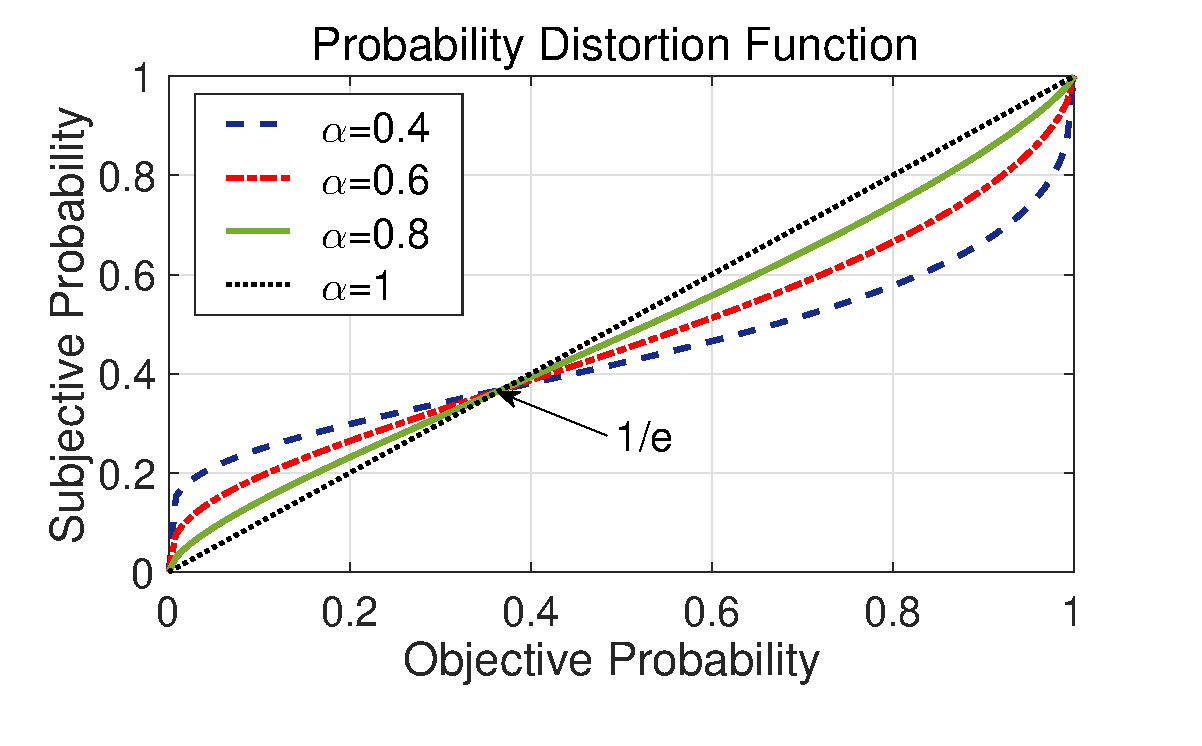
\includegraphics[scale=0.6]{./pic/dist_func.eps}
%\caption{Probability distortion functions under different distortion parameters $\alpha$.}\label{fg:dist_func}
\caption{失真参数$\alpha$不同取值下的概率失真函数。}\label{fg:dist_func}
\vspace{0.1cm}
\centering
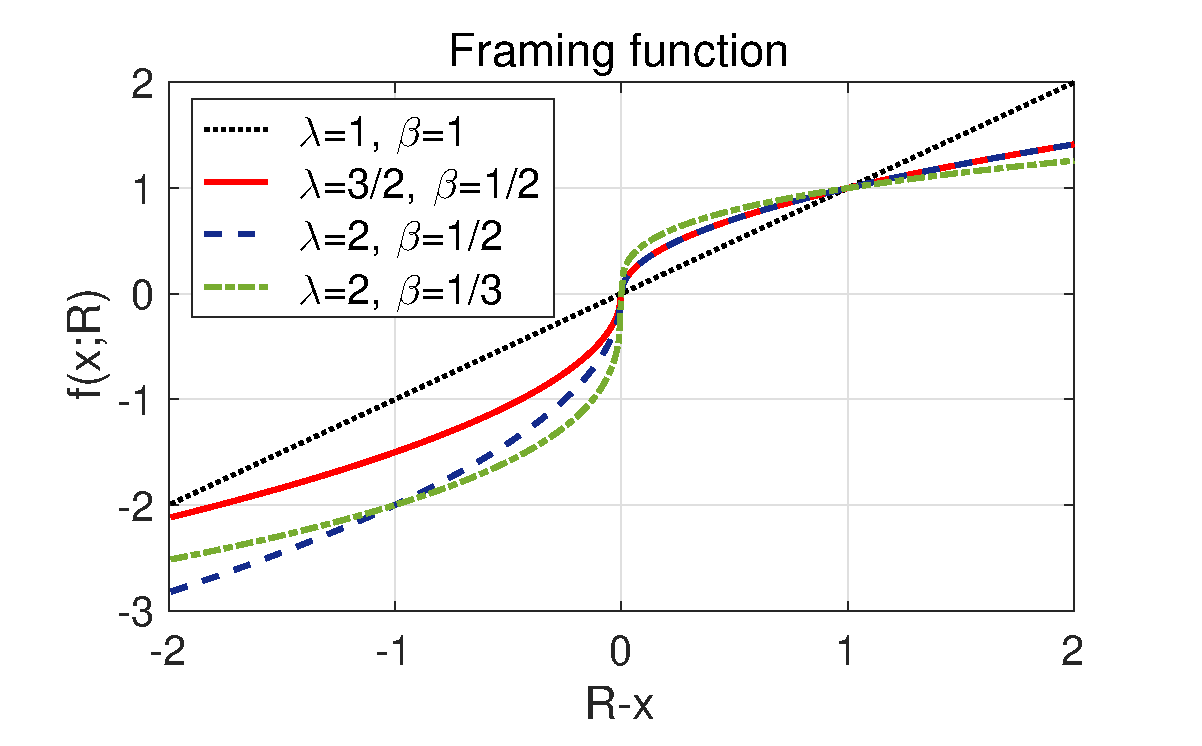
\includegraphics[scale=0.6]{./pic/fram_func.eps}
%\caption{Framing functions under different utility aversion parameters $\beta$ and loss penalty parameter $\lambda$.}\label{fg:fram_func}
\caption{不同效用规避参数$\beta$和损失惩罚参数$\lambda$下的框架函数。}\label{fg:fram_func}
\end{figure}

\subsection{效用框架效应}
我们考虑的展望理论的另一个特征是效用框架效应。此效应反映了每个服务提供商对自己的收益进行主观评估的实际情况。实际中,仅当其收入超过参照点$R$($R$无需等于零)时,每名用户才会将其视为收益增益,否则将视为收益损失。同样,在给定参考点$R$的情况下,S型单调框架函数$f(\cdot)$会进一步调整客观收入,其中函数在$v>R$侧为凹函数,而在$v<R$一侧是凸函数。此外,在$R$附近,收益损失比收益增益增长得更快,表明收益损失的边际效用大于收益增益的边际效用。常用的框架函数为Kahneman框架\cite{Kahneman},
%Another characteristic of Prospect Theory we considered is the \emph{utility framing effect}. This effect captures the practical situation where each service provider has subjective evaluation of her own payoff. In practice, each user might consider her payoff as a gain only if it is above a reference point $R$ (not necessarily equals zero), and consider it as a loss otherwise. Also, given the reference point $R$, the objective payoff is further tuned by a S-shaped monotone framing function $f(\cdot)$, which is concave at the side where $v>R$, and convex at the side where $v<R$. In addition, in the neighborhood of $R$, the losses loom larger than gains indicating that the marginal utility in losses is larger than in gains. In this work, we use a framing function based on the one proposed in \cite{Kahneman},
\begin{equation}\label{eq:framing}
f(x;R)=
\begin{cases}
(v - R)^{\beta}, &v\geq R\\
-\lambda(R-v)^{\beta}, &v<R
\end{cases}
\end{equation}
其中参数$0<\beta\leq 1$和$\lambda\geq 1$分别用于刻画风险规避和损失规避的因素。图\ref{fg:fram_func}展示了不同参数取值下的框架函数。特别地,当博弈参与者收入远离参照点时,$\beta$值越大,表示风险规避程度较小;$\lambda$值的增大则刻画了博弈参与者在客观上经历等同的收益的损失和增益时,所主观上体验到的损失要大于所体验到的增益。容易看出,当$\beta=\lambda=1$时,主观收益曲线与原始的客观收益曲线一致。
%我们假设每个服务提供商$k$基于式(\ref{eq:framing})来评估其收入。则在前景理论模型下,服务提供商$ k\in\K$的预期收入$z_k^{PT}$可写为
%where the parameters $0<\beta\leq 1$ and $\lambda\geq 1$ model the risk aversion and loss aversion respectively. Fig. \ref{fg:fram_func} illustrates the framing function with different parameters. In particular, a larger $\beta$ characterizes less degree of risk aversion when the player's payoff is away from the reference point; and a larger $\lambda$ captures the greater loss experienced by the player with her payoff being reduced by a certain amount, in comparison to the corresponding gain she experiences with the same amount of the payoff increase. It is easy to see that when $\beta=\lambda=1$, the subjective payoff boil down to the original objective payoff. We assume each service provider $k$ evaluate her revenue using (\ref{eq:framing}) with parameter $\beta_k$, and reference point $R_k, \forall k\in\K$. Under Prospect Theory model, the expected revenue $z_k^{PT}$ of service provider $k\in\K$ can be written as

%\begin{equation}\label{eq:PT}
%%\small
%z_{k}^{PT}(\pi_{k},\pi_{-k})=\sum_{\mathbf{p}\in \mathcal{P}}\pi_k(p_k)w\left(\prod_{k'\in\K,k'\neq k}\pi_{k'}(p_{k'})\right)f_k(v_k).
%\end{equation}
%
%我们将前景理论讨论下的定价博弈表示为$\mathcal{G}_P^{PT}\left(\mathcal{K},\Delta\mathcal{P},\{z_k^{PT}(R_k)\}_{k\in\mathcal{K}}\right)$,然后在下一节中重新讨论价格博弈的均衡解的存在。
%We denote the pricing game under Prospect Theory as $\mathcal{G}_P^{PT}\left(\mathcal{K},\Delta\mathcal{P},\{z_k^{PT}(R_k)\}_{k\in\mathcal{K}}\right)$, and revisit the existence of equilibrium solution for the pricing game in the next section.

展望理论在移动网络的效用优化问题研究中有着较大的应用价值。近些年,人们在解决一些移动网络中个体决策问题时,采用了展望理论对决策过程进行建模。 例如,Li等\cite{Tianming}研究了一种无线环境下的随机接入博弈,其中用户考虑了展望理论中的{\kaishu 概率失真效应}作用,策略性地确定其在冲突信道上的传输概率。Yu等\cite{Yu}研究了一种数据市场模型,模型中用户需要选择成为数据卖方还是数据买方,并确定交易的数据量。他们考虑了展望理论中的{\kaishu 概率失真效应}和{\kaishu 效用框架效应}对用户决策行为的影响,并将该问题表述为非凸优化问题。本文第五章中则运用了展望理论对无线服务提供商的有限理性行为进行刻画与建模。

%\section{本章小结}\label{chp2:sec:con}
